
\chapter{Einleitung}

\section{Motivation}

Mit Surfen oder Wellenreiten bezeichnet man eine Wassersportart, bei
der versucht wird, auf einem Surfbrett stehend eine brechende Welle
entlang zu fahren. Anders als beim Windsurfen wird hier nicht die
Kraft des Windes, sondern die Kraft der brechenden Welle benutzt, um
die zum Aufstehen und Fahren benötigte Geschwindigkeit zu
erreichen. Zum Surfen geeignete Wellen fangen idealerweise an einem
Punkt an zu brechen, und fallen dann kontinuierlich in eine oder beide
Richtungen in sich zusammen. Der Surfer versucht die Welle am
brechenden Punkt anzupaddeln, aufzustehen um dann auf der Welle so
lange wie möglich in die brechende Richtung zu fahren.

Diese Wellen sind allerdings nicht immer dort anzutreffen wo es ein
Meer oder einen Strand gibt. Vielmehr sind für Surfer interessante
Wellen an den Orten zu finden, im folgenden \textit{Spots} genannt,
deren geografische Lage das Eintreffen von oft weit entfernt
entstandenen Wellen begünstigt. Die Beschaffenheit des Untergrunds,
über dem die Wellen brechen, ist außerdem ein wichtiger Faktor, der
die Qualität der zu surfenden Wellen beeinflusst. An den bei Surfern
sehr beliebten \textit{Pointbreaks} brechen die Wellen immer an einem
bestimmten Punkt über einem Riff oder steinigem Boden. Diese sind die
beständigsten, am besten einschätzbaren, aber auch gefährlichsten
Spots.

Besteht der Untergrund aus Sand, sind meist durch Gezeiten, Strömungen
und Stürme sich ständig verändernde Sandbänke für das Brechen der
Wellen verantwortlich. Weitere wichtige Faktoren, die sich auf die
Eigenschaften von surfbaren Wellen auswirken, sind die Gezeiten, die
Richtung aus der die Wellen kommen, sowie die Wind- und
Wetterverhältnisse in den jeweiligen Jahreszeiten.

Die sogenannten \textit{Stormrider Guides} des \textit{Low Pressure}
Verlags sind seit langem die populärsten Reiseführer in der
Surfszene. Sie erfreuen sich dank der vielen hilfreichen Informationen
und Tipps einer sehr großen Beliebtheit. Die nach Kontinenten und
Ländern gegliederten Bücher enthalten Reiseinformationen über Land und
Leute, Kultur, Klima sowie Kartenausschnitte mit Beschreibungen zu den
Surfbedingungen, die an den jeweiligen Spots herrschen. Insbesondere
die detaillierten Informationen über die Eigenschaften der Wellen und
der Umgebung sind von großem Nutzen. Zum Beispiel wird beschrieben zu
welcher Gezeit bzw. \textit{Tide} die Wellen an einem Spot am besten brechen,
wie stark die Meeresströmung ist oder ob die Brandung an einem
Sandstrand oder auf einem flachen Riff ist.

% \begin{figure}[h]
%   \begin{center}
%     \includegraphics[width=450px]{bilder/stormrider-sample}
%     \caption{Beispiel aus dem World Stormrider Guide}
%   \end{center}
% \end{figure}

\section{Swell - Die Entstehung von Wellen}
Die besten Surfspots auf der Welt sind meist in den Ländern zu finden,
in denen regelmäßig \textit{Swell} eintrifft. Mit \textit{Swell} oder
\textit{Dünung} werden Seewellen bezeichnet, deren Entstehungs\-gebiet
weit entfernt ist von dem Ort an dem sie eintreffen und brechen. Swell
wird von den unterschiedlichsten Wetter\-phänomenen, wie
z.B. Wirbelstürmen, Passatwinden, Monsune und Tiefdruckgebieten
erzeugt \cite[S.15]{storm_europe_1998}. In Europa eintreffender Swell
entsteht hauptsächlich durch die Luftzirkulation in Tiefdruckgebieten
auf dem Atlantik.

\begin{figure}[h]
  \begin{center}
    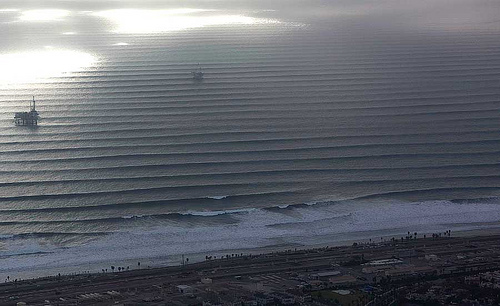
\includegraphics{bilder/swell}
    \caption{Linienförmig eintreffender Swell}
  \end{center}
\end{figure}

Wellen entstehen dadurch, dass die Wasseroberfläche durch die über ihr
strömenden Winde in Bewegung versetzt wird. Die Gipfel und Täler der
Wellen werden durch die Zirkulation des Windes über der Oberfläche
immer höher und tiefer, bis sie ein Limit erreichen und wieder in sich
zusammenbrechen. Die Höhe der Wellen ist dabei von der Stärke, der
Dauer und der Lauflänge \footnote{die Strecke über der Wind strömt}
des Windes abhängig.

Die so erzeugten Wellen breiten sich dann vom Entstehungsort
kreisförmig auf ihre Umgebung im Meer aus. Die Geschwindigkeit ist
dabei abhängig von der \textit{Wellenlänge}, dem Abstand zwischen zwei
Wellengipfeln. Das Wellenchaos am Entstehungsort mit vielen
unterschiedlichen Wellenlängen beginnt sich mit der Ausbreitung zu
legen. Die schnelleren Wellen, mit weiter auseinander liegenden
Gipfeln, beginnen die langsameren Wellen zu überholen und fangen an
sich linienförmig zu ordnen. Die vorderen Wellen werden dabei zu den
kräftiger und sauber angeordneten, die hinteren Wellen zu den
schwächeren und chaotischeren. Je weiter die Strecke die ein Swell
hinter sich gelegt hat und linienförmiger er geordnet ist, desto
größer ist die Geschwindigkeit und die Kraft der Wellen am Ort an dem
sie brechen.

Swell ist eine der Grundvoraussetzungen für gute und surfbare
Wellen. Deshalb gibt es z.B. auch in Deutschland keine guten
Surfspots, da der potentiell eintreffende Swell meistens durch England
abgeschirmt wird.

\section{Voraussetzungen zum Surfen}

\section{Ziel der Diplomarbeit}

Ziel der Diplomarbeit ist die Entwicklung einer \textit{Community
  Plattform} für Surfer, welche den Grundgedanken der
\textit{Stormrider Guides} aufgreift, mit den neuen Möglichkeiten des
Internets und des Web 2.0 verknüpft, und somit einen Mehrwert für
Surfer generiert. Grundlage der Plattform sollen Beschreibungen und
Kommentare der Mitglieder zu den verschiedenen Surf Spots sein. Diese
werden dann mit anderen Diensten wie \textit{Google Maps},
\textit{Flickr} und \textit{YouTube} verknüpft. Außerdem sollen
Wetter- und Wellenvorhersagen für die verschiedenen Spots integriert
werden, um aktuelle Informationen zu den Surfbedingungen
bereitzustellen.

Die bei der Konzeption und Implementierung aufgetretenen Probleme und
Lösungen werden in dieser Arbeit vorgestellt.


%%% Local Variables:
%%% mode: latex
%%% TeX-master: "../community-plattform"
%%% End:
